\chapter{The Trigger \& Data Acquisition}

	The Trigger system within ATLAS is designed to manage the high rate of events produced by the LHC and bring them down to a total rate that can be written to permanent storage by selecting ``interesting'' events. The related Data Acquisition (DAQ) system controls the flow of data from detector hardware through the trigger system to permanent storage at CERN and the worldwide tier 1 grid sites. 

	The Trigger system is made up of three main decision levels; Level 1, Level 2 and Event Filter. Level 1 (L1) is mainly hardware based using limited detector information to locate regions of interest (RoI's) and pass them the Level 2. The Level 2 (L2) system checks the RoIs with full detector granularity and precision and the last stage the Event Filter (EF) uses analysis reconstruction techniques to further select ``interesting'' events down to the level of 400-500 Hz. Both the L2 and EF triggers compose what is called the High-Level-Trigger (HLT) together with the event building software needed by the EF. Figure \ref{fig:triggerFlow} shows the over all trigger system and how data flows through it.

	\begin{figure}[h]
        \begin{center}
            %\includegraphics[scale=0.6]{images/}
        \end{center}
        \caption{Diagram showing the different stages of the Trigger and how they interact.}
        \label{fig:triggerFlow}
    \end{figure}


	Following is a description of each of the sections of the trigger while focusing in on the selection of electron objects that are relevant for this analysis. Following this is a discussion of how the trigger menu is formed so bandwidth can be shared between the differing physics goals as well as how ATLAS handles the continued high luminosity push of the LHC.


\section{Level-1 Trigger}

	The Level 1 (L1) trigger searches for RoI's consisting of strong signatures, i.e. high $p_{T}$, muons, electron/photons or jets. The L1 trigger also searches for events with a large missing transverse energy ($E^{miss}_{T}$) or large total transverse energy ($\Sigma E_{T}$). Due to the decision speed required only some parts of the detector can be used at L1 (and at a much coarser granularity than is possible). For muon acceptance only the RPC's and TGC's can be used while for electromagnetic clusters and jets as well as large $E^{miss}_{T}$ and $\Sigma E_{T}$ the full calorimetry system can be used. The Inner Detector can not be used in L1 decisions due to the time constraint. With a beam crossing interval of 50 ns latency is required to be less than \SI{2.5}{\us} with a target of \SI{2.0}{\us}. However half of this quota, about \SI{1.0}{\us}, is accounted for by the cable propagation of signals.

	%(- pipeline memories)
	%(- where and what these calculations are carried out on?)

	The L1Calo system uses trigger towers with a granularity reduced to roughly $0.1 \times 0.1$ in $\Delta\eta \times \Delta\phi$ in most of the detector range from both the electromagnetic and hadronic calorimeters. The ECAL produces almost 3500 of these trigger towers via summation of the analogue signals from a range of trigger cells. This trigger tower data is then sent to the Cluster Processor (CP) to identify electron/photon and tau candidates with $E_{T}$ above a required threshold and passing isolation requirements, which are labelled as RoI's.

	\begin{figure}[h]

		\begin{center}
			$\vcenter{\hbox{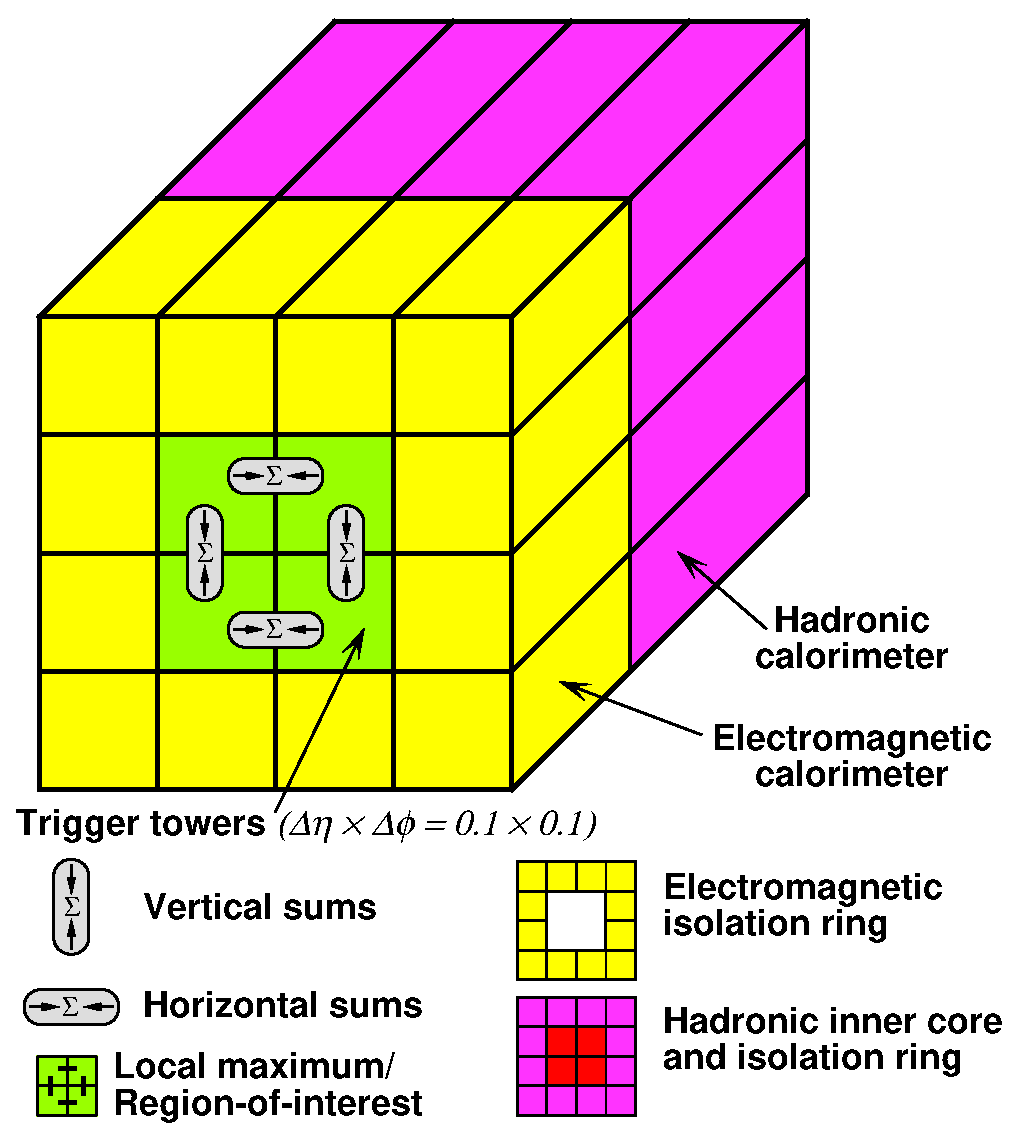
\includegraphics[scale=0.5]{images/EGammaTauAlgo.eps}}}$
			\hspace*{.5in}
			$\vcenter{\hbox{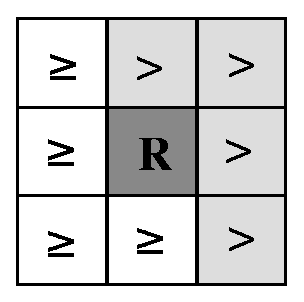
\includegraphics[scale=1.3]{images/LocalMax.eps}}}$
		\end{center}
		\caption{ Electron/photon and tau trigger algorithms (left) and E$_{T}$ local-maximum test for a cluster/RoI candidate (right). (The eta-axis runs from left to right, and the phi-axis from bottom to top. The symbol R refers to the candidate 2x2 region being tested.)  }
		\label{fig:Trig_algo}
	\end{figure}


	Figure \ref{fig:Trig_algo} shows how the electron/photon trigger clustering algorithm works by identifying $2 \times 2$ clusters of trigger towers within which two adjacent towers sum to greater than the triggering threshold defined in the trigger menu (seen in section \ref{sec:trig_menu}). Also shown is how three forms of isolation can be applied at this stage: the 12-tower surrounding ring, the $2 \times 2$ hadronic core behind the RoI and the 12-tower surrounding ring in the hadronic calorimeter. Only the hadronic core isolation has so far been used in electron/photon triggers within ATLAS. 
	As all possible $2 \times 2$ clusters are observed in this way it is possible to have double counting of RoIs and so the sum of each $2 \times 2$ RoI must be greater than each of its eight nearest overlapping neighbours. Figure \ref{fig:Trig_algo} also shows how this local-maxima is tested to avoiding identical sums through use of `greater than' and `greater than or equal to' in differing $\eta$ and $\phi$ directions. So if two adjacent $2 \times 2$ clusters have the same combined energy sum the one to the top or right is chosen so as not to delay the trigger process.
	The final L1 trigger decision is made by the Central Trigger Processor (CTP) which takes information from both the CP and jet algorithm as well as the L1 muon trigger. If an accept decision is made then RoI's are sent to the RoI builder which seeds the L2 trigger system and all L1 sub-systems are read out via Readout Drives (ROD's)(discussed in section \ref{sec:trig_DAQ}) to the DAQ system for monitoring of the L1 trigger system.



\section{Higher Level Trigger}

	\subsection*{Level-2 Trigger}

		The Level-2 (L2) trigger is seeded by and only makes decisions based on the RoI's supplied by the L1 trigger. However it does this with full detector information and so the first stage of this trigger is a RoI builder. The RoI builder requests detector information for all relevant detectors for the observed RoI, including at this level the Inner Detector. In the case of electrons this includes the inner tracking detector, the electromagnetic calorimeter and the hadronic calorimeter. It is at L2 that a distinction between electrons and photons can be made due to existence of an associated track in the ID to the RoI in the ECAL. The RoI builder identifies calorimeter clusters and nearby tracks in order for the L2 trigger to make its decision based on algorithms reconstructing shower shapes, track-cluster matching and $E_{T}$ thresholds with isolation. The list of these requirements are held within trigger chains each designed to accept specific physics signatures (see section \ref{sec:egammaMenu}). The general idea is simply to check if RoI's still exist under closer inspection in order to reduce the rate of events before full event building takes place in the Event Filter.


		%(-L2SV supervisor?, L2PU's processing unit)


	\subsection*{Event Filter}
		The Event Filter (EF) doesn't differ in method much to the L2 trigger it is purely a further test of the signals handed over from L2. At this level a full reconstruction of the event takes place and EF trigger requirements with slightly more stringent thresholds are applied to the event. This is the final decision for weather the event is going to be copied to permanent storage an so the EF reduces the final acceptance rate down to the 400 - 500 Hz require by CERN's computing systems. The requirements at the EF level are also those used in ATLAS analysis so as to treat MC and data samples the same. These requirements are discussed in section \ref{sec:egammaMenu}.
	



\section{Data Acquisition}
\label{sec:trig_DAQ}

	The Data Acquisition (DAQ) is the set of systems that control the flow of data from detectors, through the trigger and in to permanent storage. The first stage of this process is the Readout System (ROS) a set of 145 PC's or nodes which manages the collection of all detector sub-system data and L1 trigger output from ATLAS. This system is helped by Readout Drives (ROD's) which interface directly with detector components and Readout Links (ROL's), direct point-to-point readout connecting the ROD's with the ROS's. Table \ref{tab:DAQ_readouts} shows the number of readouts for each component of the detector and L1 system.


	\begin {table}[h!]
	\begin{center}
		\begin{tabular}{ | l | l | l | c | c | c | }% c | }
		\hline
\multicolumn{3}{|c|}{Detector Partition}											& Number of & Number of & Number of \\% & Data per L1A signal 	\\
\multicolumn{3}{|c|}{ }																& ROD’s 	& ROL’s 	& ROS’s 	\\% & (kbyte)				\\
		\hline
\multirow{11}{*}{Inner detector} 	& \multirow{3}{*}{Pixel} 	& Layer 0 			& 44 		& 44 		& 4 		\\% & \multirow{3}{*}{60}	\\
									&  							& Disks 			& 24 		& 24 		& 2 		\\% & 						\\
									&							& Layers 1–2 		& 64 		& 64 		& 6 		\\% &						\\
									\cline{2-6}
									& \multirow{4}{*}{SCT}		& End-cap A 		& 24 		& 24 		& 2 		\\% & \multirow{4}{*}{110}	\\
									& 							& End-cap C 		& 24 		& 24 		& 2 		\\% &						\\
									& 							& Barrel A 			& 22 		& 22 		& 2 		\\% & 						\\
									& 							& Barrel C 			& 22 		& 22 		& 2 		\\% &						\\
									\cline{2-6}
									& \multirow{4}{*}{TRT}		& End-cap A 		& 64 		& 64 		& 6 		\\% & \multirow{4}{*}{307}	\\
									& 							& End-cap C 		& 64 		& 64 		& 6 		\\% &						\\
									& 							& Barrel A 			& 32 		& 32 		& 3 		\\% & 						\\
									& 							& Barrel C 			& 32 		& 32 		& 3 		\\% & 						\\
		\hline
\multirow{10}{*}{Calorimetry}		& \multirow{4}{*}{Tile}		& Barrel A 			& 8 		& 16 		& 2 		\\% & \multirow{4}{*}{48}	\\
									& 							& Barrel C 			& 8 		& 16 		& 2 		\\% &						\\
									& 							& Extended barrel A & 8 		& 16 		& 2 		\\% &						\\
									&							& Extended barrel C & 8 		& 16 		& 2 		\\% &						\\
									\cline{2-6}
									& \multirow{6}{*}{LAr}		& EM barrel A 		& 56 		& 224 		& 20 		\\% & \multirow{6}{*}{576}	\\
									& 							& EM barrel C 		& 56 		& 224 		& 20 		\\% &						\\
									& 							& EM end-cap A 		& 35 		& 138 		& 12 		\\% &						\\
									& 							& EM end-cap C 		& 35  		& 138 		& 12 		\\% &						\\
									&							& HEC 				& 6 		& 24 		& 2 		\\% &						\\
									& 							& FCal 				& 4 		& 14 		& 2 		\\% &						\\
		\hline
\multirow{6}{*}{Muon spectrometer}	& \multirow{4}{*}{MDT}		& Barrel A 			& 50 		& 50 		& 4 		\\% & \multirow{4}{*}{154}	\\
									& 							& Barrel C 			& 50 		& 50 		& 4 		\\% &						\\
									& 							& End-cap A 		& 52 		& 52 		& 4  		\\% &						\\
									& 							& End-cap C 		& 52 		& 52 		& 4 		\\% &						\\
									\cline{2-6}
									& \multirow{2}{*}{CSC} 		& End-cap A 		& 8 		& 8 		& 1 		\\% & \multirow{2}{*}{10}	\\
									&							& End-cap C 		& 8 		& 8 		& 1 		\\% &						\\
		\hline
\multirow{9}{*}{L1}					& \multirow{3}{*}{Calorimeter} & CP				& 4 		& 8 		& 1  		\\% & \multirow{2}{*}{28 (can be varied)} \\
									& 							& JEP 				& 2 		& 8 		& 1 		\\% &						\\
									& 							& PP 				& 8 		& 32 		& 3 		\\% &						\\
									\cline{2-6}
									& \multirow{2}{*}{Muon RPC} & Barrel A 			& 16 		& 16 		& 2 		\\% & \multirow{2}{*}{12} 	\\
									& 							& Barrel C 			& 16 		& 16 		& 2 		\\% &						\\
									\cline{2-6}
									& \multirow{2}{*}{Muon TGC} & End-cap A 		& 12 		& 12 		& 1 		\\% & \multirow{2}{*}{6}	\\
									& 							& End-cap C 		& 12 		& 12 		& 1 		\\% & 						\\
									\cline{2-6}
									& \multicolumn{2}{c|}{MUCTPI} 					& 1 		& 1 		& 1 		\\% & 0.1					\\
									& \multicolumn{2}{c|}{CTP}						& 1 		& 1 		& 1 		\\% & 0.2					\\
		\hline
\multicolumn{3}{|r|}{Total}															& 932 		& 1574 		& 145 		\\% & 1311					\\
    	\hline
  		\end{tabular}
  	\caption{Numbers of readout drivers (ROD’s), readout links (ROL’s) and readout systems (ROS’s) per detector partition \cite{Aad:1129811}.}%, as well as expected data size per L1A signal for a luminosity of 1034 cm$^{-2}$ s$^{−1}$.}
  	\label{tab:DAQ_readouts}
  	\end{center}
	\end {table}


  	Each ROS PC contains Readout Buffer Module's (ROBIN's), custom PCI-X cards, each containing three Readout Buffers (ROB's), the other end of each ROL. The ROB's is where event data is stored while the L2 trigger makes its decision which comes from the set of 10 L2 Supervisor (L2SV) nodes. This decision is then made by the DataFlow Manager (DFM) on input from all the L2SV nodes and sends a command to the ROS's to either expunge data or forward it on to the event building nodes (or Sub farm Input, SFI). Once a event fully built it is sent forward to the HLT farm which makes the EF decision, then and only then is a message sent back down via the DFM for the ROS's to fully delete all data from the event. The HLT farm is the largest computing resource in the DAQ system with 1116 nodes each containing 8 CPU's. These nodes can either be configured to run as the EF or L2 Processing Units (L2PU's) for the L2SV and are reconfigured as need dictates. As the final step if an event is accepted by the EF all data is passed to the Sub Farm Output (SFO) where it is stored before transfer to CERN's central data-recording facility. In the case that this connection to CERN is offline for some reason ATLAS is able to store about 24 hours worth of data in the SFO's so no data is lost.
  	Table \ref{tab:DAQ_comp} shows the number of each DAQ component used within ATLAS all of which are found in the USA15 service cavern next to the ATLAS cavern.


	\begin {table}[h!]
	\begin{center}
  	\begin{tabular}{ | l | c | c | c | }%c | c | }
		\hline
		Component & Number of & Number of & Number of \\%& Memory (Gbyte) & Type of CPU \\
		& nodes & racks & CPU’s/node \\
		\hline 
		ROS & 145 & 16 & 1 \\%& 0.512 & 3.4 GHz Irwindale \\
		\hline
		DFM & 12 & 1 & 2 \\%& 2 & 2.6 GHz Opteron 252 \\
		L2SV & 10 & 1 & 2 \\%& 2 & 2.6 GHz Opteron 252 \\
		SFI & 48 & 3 & 2 \\%& 2 & 2.6 GHz Opteron 252 \\
		HLT & 1116 & 36 & 8 \\%& 8 & Xeon E5320 1.86 GHz \\
		SFO & 6 & 2 & 2 \\%& 4 & Xeon E5130 2.0 GHz \\
		\hline
		Monitoring & 32 & 4 & 4 \\%& 8 & Xeon E5160 3.0 GHz \\
		Operations & 20 & 4 & 2 \\%& 4 & Xeon E5130 2.0 GHz \\
    	\hline
  	\end{tabular}
  	\caption{The main data-acquisition system components to be deployed for initial operation: the readout system (ROS), the event-building node (SFI), the data flow manager (DFM), the L2 supervisor (L2SV), the high-level trigger (HLT) and the event filter output nodes (SFO) \cite{Aad:1129811}.}
  	\label{tab:DAQ_comp}
  	\end{center}
	\end {table}


\section{Trigger Menu and Rates}
\label{sec:trig_menu}

	In its simplest form a single trigger is a energy threshold designed to select a high quantity of particles of of a selected type. ATLAS contains many of these thresholds to select many interesting physics objects which are roughly grouped in to similar signatures called streams. The trigger streams are Egamma triggers to select electrons and photons, JetTauEtMiss triggers to select hadronic decays, tau decays and large missing transverse energy, Muon triggers to select muons, MinBias trigger to check no bias's exist in other triggers and cosmics triggers to selected signals of cosmic radiation. Each stream has a given bandwidth allocated for readout from the trigger so all triggers need to be optimised so total acceptance rates are within requirements. Each trigger at the HLT level is designed to select a specific type of signal while those a L1 are more general and seed many HLT triggers. A full run through all three stages of the trigger is called a trigger chain. Each trigger in a trigger chain needs to not only be optimised to fulfil acceptance rate but also optimised to for high acceptance efficiency in the valid region. In terms of energy threshold this means an increasing threshold through the trigger chain so that each level is selecting within the range close to $100\%$ efficient from the previous requirement when taking in to account the different accuracy of energy measurement provided by each level. This section focuses on the Egamma trigger stream as all objects in this analysis where selected using it.

	%-jets stream used in the fake rates method?


	\subsection{The ``$e/\gamma$'' Trigger Menu} 
		\label{sec:egammaMenu}

		The $e/\gamma$ trigger menu that is used in this analysis refers to trigger chains designed to select electron and photon objects detailing requirements for all three stages of the trigger. ATLAS uses its own terminology to name these triggers with the name giving a description of the requirements used. At L1 electron and photon objects are selected with bearing the name EMXY where; `EM' refers to EM calorimeter, X is the value of the energy threshold required of RoIs in GeV and Y refers to any other specification. Other specifications can be `V' is a threshold varying in detector geometry ($\eta$) around the given value to optimise selection or `H' indicating hadronic isolation applied behind the RoI, both of which are discussed in section \ref{sec:TrigRates}. An example of a L1 trigger is then L1\_EM16VH which is a trigger with an energy threshold of 16 GeV which is varied slightly through the detector and has an hadronic isolation requirement. L2 and EF use the same terminology but are prepended with either L2 or EF. They take the form such as e22vh\_medium where `e' represents an electron (g is used for photons), `vh' represents the same as above and `medium' refers to an associated set of shower shape and tracking requirements. As well as `medium', `loose' and `tight' are also defined giving looser and tighter requirements respectively. These shower shape and tracking requirements are discussed in section \ref{sec:ReconElec}. Section \ref{sec:TrigRates} discusses the development of the L1\_EM16VH trigger which feeds in to L2\_e20vh\_medium and then in to EF\_e22vh\_medium. 

		The analysis discussed in the rest of this thesis uses a photon trigger even though searching for electrons. This is because photon and electron triggers are identical save for tracking requirements for electrons and it turned out for the 2012 run the lowest energy triggers without hadronic isolation that were applicable for high energy dielectron decays was a diphoton trigger chain. It is important that the trigger used did not have hadronic isolation due to the very high energy nature of the electrons in this analysis which have a higher chance of leaking through in to the hadronic calorimeter. The trigger used is EF\_g35\_loose\_g25\_loose which selects two photon objects with thresholds of 35 GeV and 25 GeV while both requiring `loose' shower shape requirements. This trigger is seeded by L2\_g30\_loose\_g20\_loose which itself is seeded by L1\_2EM12\_EM16V.



	\subsection{Trigger Rates in High Luminosity Regime}
		\label{sec:TrigRates}

		The ATLAS trigger system comprises a hardware-based Level-1 (L1) trigger and a software-based High Level Trigger (HLT), subdivided into the Level-2 (L2) and Event Filter (EF). Due to the bandwidth limitations of the trigger each level is restricted to a certain output rate. During 2011 the L1 output rate was kept below 60 kHz, L2 below 5 kHz and the EF output rate at around 400 Hz averaged over the LHC fills. The bandwidth allocated to the $e/\gamma$ triggers was approximately 30\% of the total EF output rate. Electron and photon identification is accomplished by a set of $\eta$- and $E_{T}$-dependent rectangular cuts variables \cite{trig1, trig2}.\\
		Throughout 2011 data taking at ATLAS the luminosity continued to increase putting pressure on the trigger's ability to control the output rate. Several methods were employed to reduce the trigger rate and in the $e/\gamma$ trigger a variable threshold and hadronic core isolation was investigated to reduce the rate of the Level-1 trigger. In order to keep within time constraints only a coarse granularity is available Level-1 trigger in regions of 0.4 $\eta$. Threshold requirements were therefore investigated varying every 0.4 $\eta$. The effect of a hadronic core isolation was also investigated on the selection of electrons which defines a region in the hadronic calorimeter behind the $e/\gamma$ candidate in which you require and minimum amount of energy to be deposited to distinguish between jets and $e/\gamma$ objects. 


		\begin{figure}[h!]
			\centering
				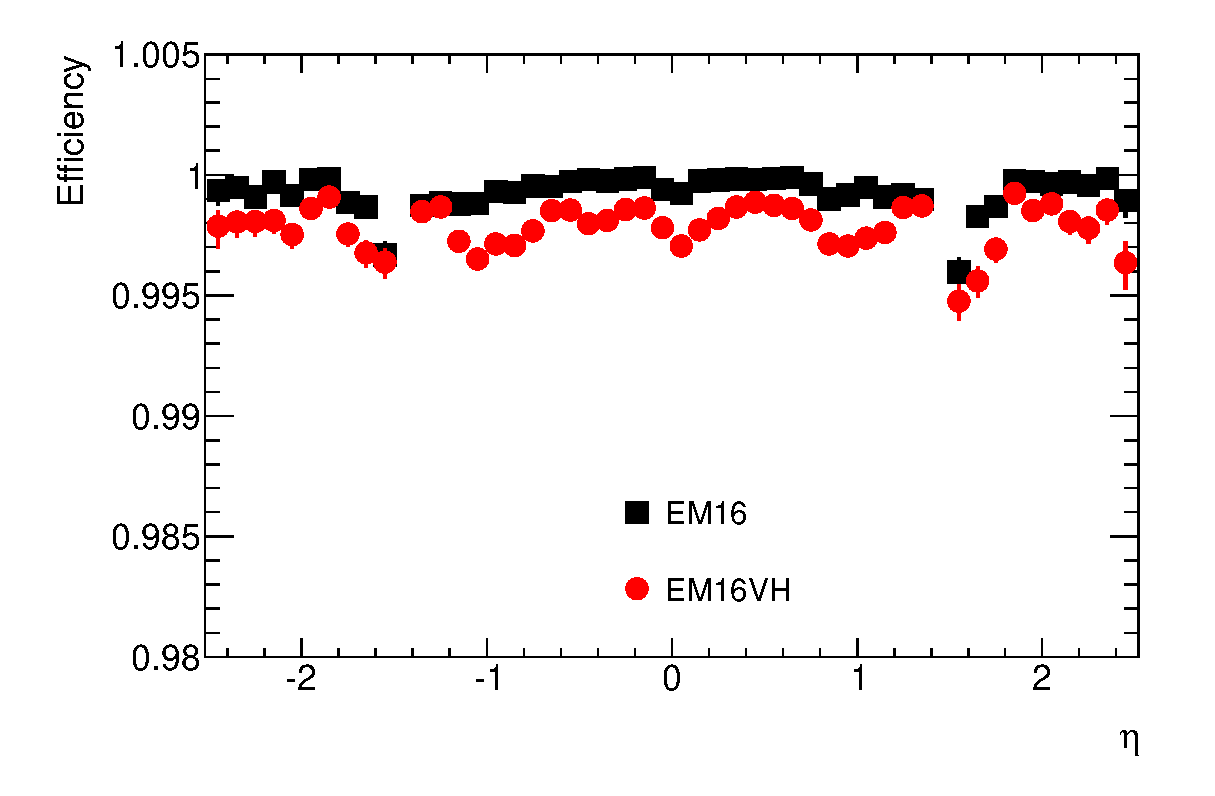
\includegraphics[width=0.49\linewidth]{images/L1_EM16VH_TandP_eff_vs_eta.eps}
				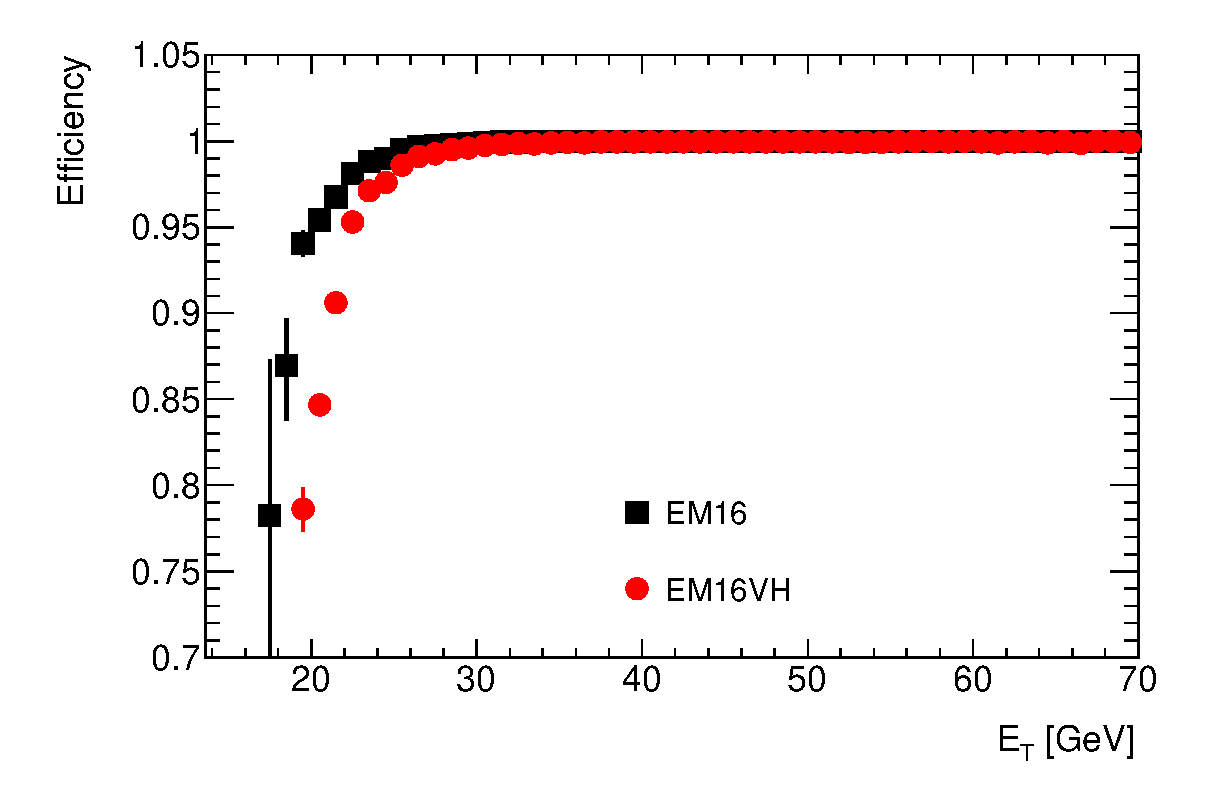
\includegraphics[width=0.49\linewidth]{images/L1_EM16VH_TandP_eff_vs_Et.eps}

				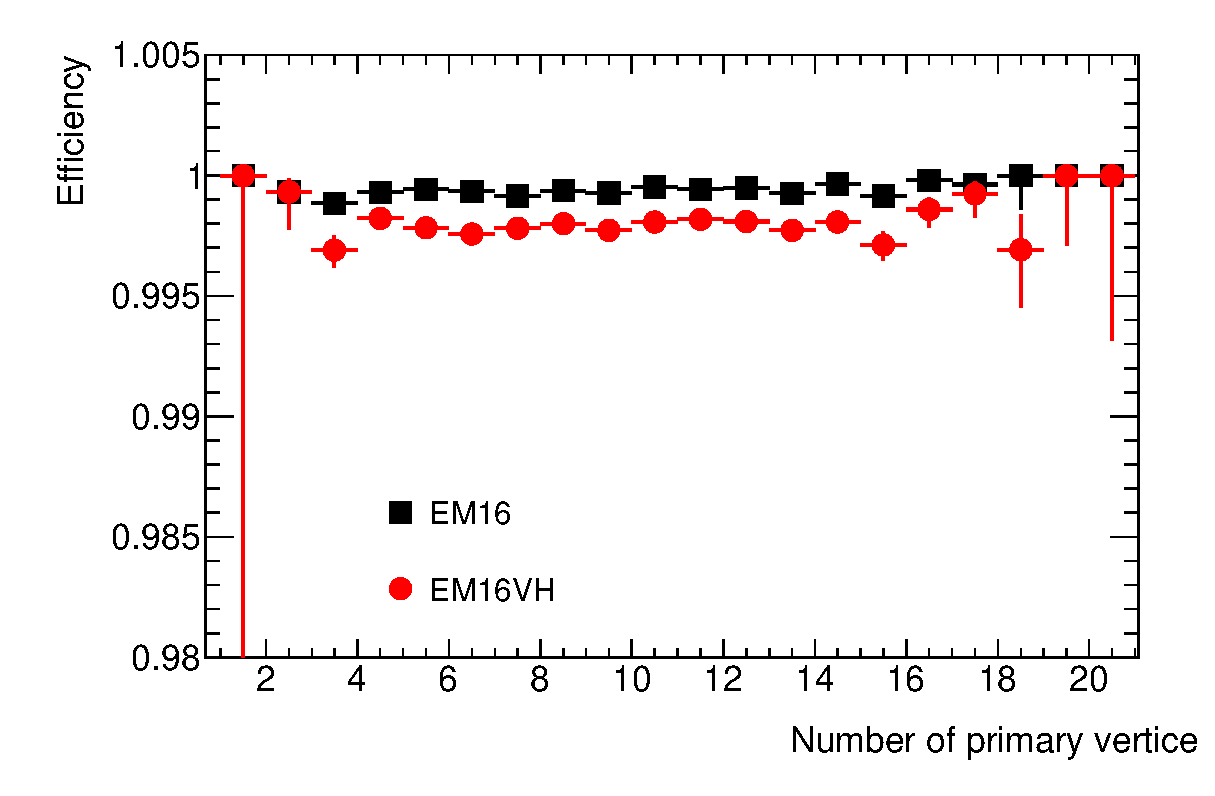
\includegraphics[width=0.49\linewidth]{images/L1_EM16VH_TandP_eff_vs_pvx.eps}
			\caption{Performance of the first level of the ATLAS $e/\gamma$ trigger before(EM16) and after(EM16VH) variable thresholds and hadronic core isolation are applied.}
			\label{fig:L1}
		\end{figure}

		These attempts where successful and rate reduced to compensate for the high luminosity environment. Fig. \ref{fig:L1} shows the performance of the trigger after these changes had been made. It can be seen that a minimal impact of these new requirements is felt.


		There was also a contribution to the maintenance of the $e/\gamma$ trigger software run in the ATLAS detector, both these tasks forming the authorship qualification. The authorship task culminated in presentation of a poster on behalf of the $e/\gamma$ trigger group at the Computing and High Energy Physics (CHEP) conference held New York in May 2012. The contribution is included two pages previously and details the performance of the $e/\gamma$ trigger in the 2011 run period \cite{poster}.

